%% ============================================================
%%  TALLER 1 - CONTROL ROBUSTO: VEHICULO AEREO NO TRIPULADO
%%  Compilar con: pdflatex  (Overleaf funciona tal cual)
%% ============================================================
\documentclass[11pt,letterpaper]{article}

% ---------- Codificacion e idioma ----------
\usepackage[utf8]{inputenc}
\usepackage[T1]{fontenc}
\usepackage[spanish,es-noshorthands,es-tabla]{babel}
\usepackage{lmodern}
\usepackage{microtype}

% ---------- Pagina ----------
\usepackage[top=2.5cm,bottom=2.3cm,left=2.3cm,right=2.3cm,headheight=28pt]{geometry}
\usepackage{fancyhdr}
\usepackage{lastpage}
\usepackage{setspace}
\setstretch{1.12}

% ---------- Matematicas ----------
\usepackage{amsmath,amssymb,mathtools}
\usepackage{siunitx}
\sisetup{output-decimal-marker={,}}

% ---------- Graficos y tablas ----------
\usepackage{graphicx}
\usepackage{xcolor}
\usepackage{booktabs}
\usepackage{array}
\usepackage{multirow}
\usepackage{tabularx}
\usepackage{float}
\usepackage[font=small,labelfont=bf]{caption}
\usepackage{subcaption}
\usepackage{tcolorbox}
\tcbuselibrary{skins,breakable}
\graphicspath{{Imagenes/}}

% ---------- Codigo MATLAB ----------
\usepackage{listings}

\definecolor{mlkeyword}{RGB}{0,0,255}
\definecolor{mlcomment}{RGB}{0,128,0}
\definecolor{mlstring}{RGB}{160,32,240}
\definecolor{mlbg}{RGB}{248,248,248}

\lstdefinestyle{matlabstyle}{
  language=Matlab,
  basicstyle=\ttfamily\footnotesize,
  keywordstyle=\color{mlkeyword}\bfseries,
  commentstyle=\color{mlcomment}\itshape,
  stringstyle=\color{mlstring},
  numbers=left,
  numberstyle=\tiny\color{gray},
  numbersep=8pt,
  backgroundcolor=\color{mlbg},
  frame=single,
  rulecolor=\color{black!25},
  breaklines=true,
  breakatwhitespace=false,
  tabsize=4,
  showstringspaces=false,
  columns=fullflexible,
  keepspaces=true,
  xleftmargin=14pt,
  captionpos=b,
  literate=
    {a}{{\'{a}}}1 {e}{{\'{e}}}1 {i}{{\'{i}}}1 {o}{{\'{o}}}1 {u}{{\'{u}}}1
    {A}{{\'{A}}}1 {E}{{\'{E}}}1 {I}{{\'{I}}}1 {O}{{\'{O}}}1 {U}{{\'{U}}}1
    {n}{{\~{n}}}1 {N}{{\~{N}}}1
}

\lstset{style=matlabstyle}
\renewcommand{\lstlistingname}{C\'{o}digo}

\lstdefinestyle{salida}{
  style=matlabstyle, language={}, numbers=none,
  backgroundcolor=\color{white}, frame=leftline,
  commentstyle=\color{black}, xleftmargin=6pt
}

% ---------- Listas y enlaces ----------
\usepackage{enumitem}
\setlist[enumerate,1]{label=\textbf{\arabic*.},leftmargin=*}
\setlist[enumerate,2]{label=\textbf{\alph*)},leftmargin=1.8em}
\usepackage[hidelinks]{hyperref}

% ============================================================
%  DATOS DEL TRABAJO
% ============================================================
\newcommand{\universidad}{Universidad Nacional de Colombia}
\newcommand{\facultad}{Facultad de Ingenier\'{\i}a}
\newcommand{\departamento}{Departamento de Ingenier\'{\i}a Mec\'anica y Mecatr\'onica}
\newcommand{\programa}{Ingenier\'{\i}a Mecatr\'onica}
\newcommand{\curso}{Teor\'{\i}a de Control}
\newcommand{\tipo}{Taller N.\textsuperscript{o}~1}
\newcommand{\profesor}{Prof.\ Jorge Iv\'an Sofrony Esmeral}
\newcommand{\periodo}{2026-II}
\newcommand{\fecha}{8 de octubre de 2026}

\newcommand{\nombregrupo}{La banda del club de los corazones solitarios del Sargento Pepper}

% Integrantes
\newcommand{\integranteA}{Samuel David Negrete Lancheros}
\newcommand{\integranteB}{Jes\'us David S\'anchez Cobos}
\newcommand{\integranteC}{Leonardo Acevedo Monroy}
\newcommand{\integranteD}{Ariel C\'ardenas}

% Correos (completar)
\newcommand{\correoA}{\textit{correo@unal.edu.co}}
\newcommand{\correoB}{\textit{correo@unal.edu.co}}
\newcommand{\correoC}{\textit{correo@unal.edu.co}}
\newcommand{\correoD}{\textit{correo@unal.edu.co}}

% ============================================================
%  ENCABEZADO Y PIE
% ============================================================
\pagestyle{fancy}
\fancyhf{}
\lhead{\small\textbf{\curso}}
\chead{\small\tipo}
\rhead{\small\periodo}
\lfoot{\small\departamento{} -- \programa}
\rfoot{\small P\'agina~\thepage\ de~\pageref{LastPage}}
\renewcommand{\headrulewidth}{0.4pt}
\renewcommand{\footrulewidth}{0.4pt}

% ============================================================
%  MACROS
% ============================================================
\newcommand{\pts}[1]{\hfill\textcolor{gray}{\small\textbf{[#1~pts]}}}
\newcommand{\dd}{\,\mathrm{d}}
\DeclarePairedDelimiter{\abs}{\lvert}{\rvert}
\DeclarePairedDelimiter{\norm}{\lVert}{\rVert}

\newtcolorbox{enunciado}{
  enhanced, breakable, colback=blue!4, colframe=blue!50!black,
  boxrule=0.5pt, arc=3pt, left=6pt, right=6pt, top=4pt, bottom=4pt,
  title=Enunciado, fonttitle=\small\bfseries
}

\newcommand{\desarrollo}{\subsection*{Desarrollo}}
\newcommand{\implementacion}{\subsection*{Implementaci\'on en MATLAB}}
\newcommand{\resultados}{\subsection*{Resultados}}
\newcommand{\analisis}{\subsection*{An\'alisis}}

\newcommand{\figura}[4]{%
  \begin{figure}[H]
    \centering
    \includegraphics[width=#2\linewidth]{#1}
    \caption{#3}\label{#4}
  \end{figure}}

\newcommand{\codigom}[3]{%
  \lstinputlisting[caption={#2},label={#3}]{#1}}

\numberwithin{equation}{section}
\setlength{\parindent}{0pt}
\setlength{\parskip}{0.6em}

% ============================================================
\begin{document}

% ---------- Portada ----------
\begin{center}
  {\large\bfseries \universidad}\\[2pt]
  {\normalsize \facultad}\\[1pt]
  {\normalsize \departamento}\\[1pt]
  {\normalsize \programa}\\[10pt]
  %
\includegraphics[width=0.18\linewidth]{LogoUnalpng.png}\\[8pt]
  {\Large\bfseries \curso}\\[2pt]
  {\large \tipo}\\[14pt]
  \begin{tcolorbox}[enhanced, colback=black!4, colframe=black!60,
      boxrule=0.6pt, arc=3pt, width=\linewidth, halign=center]
    {\LARGE\bfseries \nombregrupo}
  \end{tcolorbox}
\end{center}

\vspace{0.3cm}

% ---------- Integrantes ----------
\begin{center}
\renewcommand{\arraystretch}{1.5}
\begin{tabularx}{\linewidth}{
    >{\centering\arraybackslash}X
    >{\centering\arraybackslash}X
    >{\centering\arraybackslash}X
    >{\centering\arraybackslash}X}
  \toprule
  \textbf{\integranteA} &
  \textbf{\integranteB} &
  \textbf{\integranteC} &
  \textbf{\integranteD} \\[2pt]
  \correoA & \correoB & \correoC & \correoD \\
  \bottomrule
\end{tabularx}
\end{center}

\begin{center}
  \small \profesor \quad$\bullet$\quad \periodo \quad$\bullet$\quad \fecha
\end{center}

\vspace{0.1cm}
\hrule
\vspace{0.4cm}

% ============================================================
\section*{Introducci\'on}
% ============================================================

El presente taller aborda el dise\~no y comparaci\'on de dos estrategias de control para un \textbf{Veh\'iculo A\'ereo No Tripulado (UAV)}: un controlador cl\'asico tipo $PI+D$ basado en el esquema SAS/CAS, y un controlador robusto $\mathcal{H}_\infty$. El objetivo central es el \textit{seguimiento de referencias de posici\'on angular} (\textit{set-point tracking}) en el rango $[-40^\circ, 40^\circ]$ para los \'angulos de cabeceo~$\theta$ y alabeo~$\phi$, garantizando al mismo tiempo rechazo de ruido de medici\'on e incertidumbre aditiva inversa.

La planta corresponde a un modelo lineal nominal de UAV. El eje \textbf{lateral/direccional} tiene como entradas el aler\'on~$\delta_a$ y el tim\'on de direcci\'on~$\delta_r$, y como salidas el alabeo~$\phi$, la gui\~nada~$\psi$ y sus tasas~$(r,p)$. El eje \textbf{longitudinal} tiene como entrada el elevador~$\delta_e$ y como salida el \'angulo de cabeceo~$\theta$ y su tasa~$q$. Los ejes se tratan como desacoplados para el dise\~no y acoplados para la simulaci\'on.

Las \textbf{especificaciones de dise\~no} son:
\begin{itemize}[leftmargin=*,noitemsep]
  \item \textbf{Seguimiento:} ancho de banda m\'inimo $\omega_{BW} \geq 8\,\text{Hz}$; referencia de velocidad angular nula.
  \item \textbf{Robustez:} rechazo de perturbaciones de entrada hasta $\omega_{p,\max} = 6\,\text{Hz}$.
  \item \textbf{Rechazo de ruido:} ruido blanco con potencia $0{,}001$ (eje lateral/direccional) y $0{,}0001$ (eje longitudinal).
  \item \textbf{Esfuerzo de control:} se\~nal m\'inima posible, $|\delta| \leq 30^\circ$.
  \item Sistema cr\'iticamente amortiguado y ejes desacoplados.
\end{itemize}

\vspace{0.2cm}
\hrule
\vspace{0.3cm}

% ============================================================
\section{Dise\~no de controladores \texorpdfstring{$PI+D$}{PI+D}}
% ============================================================

El dise\~no de los controladores $PI+D$ se lleva a cabo con el esquema de control SAS/CAS.

\begin{figure}[H]
    \centering
    
\includegraphics[width=0.6\linewidth]{SAS_CAS.png}
    \caption{Esquema de control SAS/CAS.}
    \label{fig:SAS_CAS}
\end{figure}

Con este esquema, el \textbf{SAS} (\textit{Stability Augmentation System}) genera amortiguamiento realimentando la tasa angular con ganancia proporcional~$K_\text{SAS}$, moviendo los polos poco amortiguados al semiplano izquierdo y separando la acci\'on derivativa del error para evitar picos grandes en la se\~nal de control. Una vez estabilizado el lazo interno, el \textbf{CAS} (\textit{Command Augmentation System}) agrega un controlador PI para seguir el \textit{setpoint} con error nulo en estado estacionario. La estructura general del controlador es:

\begin{equation}
  C(s) = C_\text{Lead}(s)\cdot C_\text{PI}(s), \quad
  C_\text{PI}(s) = K_p\frac{s+a}{s}, \quad
  C_\text{Lead}(s) = \frac{1+b\,T_2\,s}{1+T_2\,s},\quad b>1
  \label{eq:controlador_pid}
\end{equation}

donde la \textbf{red de adelanto de fase} $C_\text{Lead}$ se sintoniza para alcanzar la frecuencia de cruce $\omega_c$ con margen de fase $\phi_m > 30^\circ$.

% -----------------------------------------------------------
\subsection{Dise\~no para eje longitudinal}
% -----------------------------------------------------------

\desarrollo

El modelo longitudinal reducido utiliza los estados $[\alpha,\,q]^T$ y la salida de inter\'es es el \'angulo de cabeceo $\theta$ (integraci\'on de $q$). El SAS realimenta $q$ con ganancia:
\begin{equation}
  D_\text{long} = -0{,}469
\end{equation}
Sobre el lazo interno estabilizado, el PI se sintoniza con:
\begin{equation}
  K_{p,\text{long}} = -14, \quad K_{i,\text{long}} = -68\,\text{rad/s}
\end{equation}
La red de adelanto se dimensiona para $\omega_c = 29{,}5\,\text{rad/s}$.

\resultados
% \figura{bode_long}{0.85}{Diagrama de Bode -- lazo abierto longitudinal.}{fig:bode_long}
% \figura{step_long}{0.85}{Respuesta al escal\'on -- canal longitudinal.}{fig:step_long}

\analisis

% -----------------------------------------------------------
\subsection{Dise\~no para eje direccional (Yaw)}
% -----------------------------------------------------------

\desarrollo

El canal direccional regula $\psi$ mediante $\delta_r$. El SAS realimenta la tasa de gui\~nada $r$:
\begin{equation}
  k_r = -0{,}174
\end{equation}
El PI se sintoniza con cero $a_\text{yaw} = 2\,\text{rad/s}$:
\begin{equation}
  K_{p,\text{yaw}} = -1{,}62, \quad K_{i,\text{yaw}} = K_{p,\text{yaw}}\cdot a_\text{yaw} = -3{,}24\,\text{rad/s}
\end{equation}
La red de adelanto se sintoniza para $\omega_c = 30\,\text{rad/s}$.

\resultados
% \figura{bode_yaw}{0.85}{Diagrama de Bode -- lazo abierto direccional.}{fig:bode_yaw}
% \figura{step_yaw}{0.85}{Respuesta al escal\'on -- canal direccional.}{fig:step_yaw}

\analisis

% -----------------------------------------------------------
\subsection{Dise\~no para eje lateral (Roll)}
% -----------------------------------------------------------

\desarrollo

El canal lateral controla $\phi$ mediante $\delta_a$. El SAS realimenta la tasa de alabeo $p$:
\begin{equation}
  K_\text{roll} = -0{,}106
\end{equation}
La ganancia $K_p$ del PI se obtiene maximiz\'andola tal que todos los polos del lazo cerrado permanezcan en el semiplano izquierdo (lugar de ra\'ices). El cero del PI es $a_\text{roll} = 0{,}0195\,\text{rad/s}$ y la red de adelanto se sintoniza para $\omega_c = 5\,\text{rad/s}$.

\resultados
% \figura{bode_roll}{0.85}{Diagrama de Bode -- lazo abierto lateral.}{fig:bode_roll}
% \figura{step_roll}{0.85}{Respuesta al escal\'on -- canal lateral.}{fig:step_roll}

\analisis

% -----------------------------------------------------------
\subsection{An\'alisis de sensibilidad -- \texorpdfstring{$PI+D$}{PI+D}}
% -----------------------------------------------------------

Para evaluar el desempe\~no nominal y la robustez con los controladores $PI+D$ se analizan:
\begin{equation}
  S(s) = \frac{1}{1+L(s)}, \quad
  T(s) = \frac{L(s)}{1+L(s)}, \quad
  K(s)S(s) = \frac{K(s)}{1+L(s)}
  \label{eq:sensibilidades}
\end{equation}
donde $L(s)=K(s)G(s)$ es el lazo abierto. El m\'aximo valor singular de cada funci\'on se obtiene con \texttt{sigma} de MATLAB para estimar la norma $\mathcal{H}_\infty$ del sistema y verificar las especificaciones de robustez.

% ============================================================
\section{Dise\~no de controladores \texorpdfstring{$\mathcal{H}_\infty$}{H-infinito}}
% ============================================================

El dise\~no $\mathcal{H}_\infty$ sintetiza un controlador $K(s)$ que minimiza la norma $\mathcal{H}_\infty$ del sistema en lazo cerrado ponderado mediante la configuraci\'on de sensibilidad mixta (\textit{mixed-sensitivity}):
\begin{equation}
  \min_{K\,\text{estabilizante}} \bigl\|\mathbf{F}_\ell(P_g,K)\bigr\|_\infty \leq \gamma, \quad
  P_g(s) = \begin{bmatrix} W_1 S_0 \\ W_2 K S_0 \\ W_3 T_0 \end{bmatrix}, \quad
  W_i(s) = \frac{\frac{1}{M_i}s + \omega_{bi}}{s + A_i\,\omega_{bi}}
  \label{eq:hinf_general}
\end{equation}
donde $S_0 = (I+GK)^{-1}$ y $T_0 = GK(I+GK)^{-1}$. La selecci\'on de filtros cumple:
\begin{itemize}[leftmargin=*,noitemsep]
  \item $W_1(s)$ (error $S$): filtro pasa-bajas; impone error en estado estacionario $1/A_1$, ancho de banda $\omega_{b1}$ y cota de pico $\|S\|_\infty \leq M_1$.
  \item $W_2(s)$ (control $KS$): penaliza el esfuerzo de actuaci\'on para impedir la saturaci\'on ($|\delta| \leq 30^\circ$).
  \item $W_3(s)$ (salida $T$): filtro pasa-altas con cota $1/A_3$ y corte $\omega_{b3}$; asegura rechazo de ruido de alta frecuencia y estabilidad robusta ante din\'amicas no modeladas.
\end{itemize}
La s\'intesis se ejecuta mediante \texttt{augw} y \texttt{hinfsyn} de MATLAB sobre los modelos desacoplados.

% -----------------------------------------------------------
\subsection{Dise\~no para eje longitudinal}
% -----------------------------------------------------------

\desarrollo
El modelo longitudinal utiliza como entrada el elevador $\delta_e$ y como medidas vectoriales la tasa $q$ y el cabeceo $\theta$ ($y = [q, \theta]^T$). La referencia se aplica exclusivamente en cabeceo ($r_\theta \in [-40^\circ, 40^\circ]$) con $r_q = 0$. Los filtros de ponderaci\'on fijados son:
\begin{equation}
  W_1 = \operatorname{diag}(0,\, W_{1\theta}),\ W_{1\theta} = \frac{0{,}333\,s + 1}{s + 0{,}001}; \quad
  W_2 = 60; \quad
  W_3 = \operatorname{diag}(0,\, W_{3\theta}),\ W_{3\theta} = \frac{50\,s + 502{,}7}{s + 502{,}7}
\end{equation}
con $M_1 = 3$, $A_1 = 10^{-3}$, $\omega_{b1} = 1\,\text{rad/s}$, $M_3 = 0{,}02$, $A_3 = 1$ y $\omega_{b3} = 2\pi(80)\,\text{rad/s}$.

\resultados
La s\'intesis converge con $\gamma = 58{,}12$, produciendo un controlador MISO de orden 8. La respuesta temporal no presenta sobrepaso ($M_p = 0{,}00\%$), con $t_r = 36{,}03\,\text{s}$ y $t_s = 74{,}09\,\text{s}$. En frecuencia se obtiene $\omega_{BW} = 0{,}0609\,\text{rad/s}$ ($0{,}0097\,\text{Hz}$), con normas pico $\|S_\theta\|_\infty = 1{,}2090$, $\|KS\|_\infty = 0{,}9652$ y $\|T_\theta\|_\infty = 0{,}9952$.

\begin{figure}[H]
  \centering
  \begin{subfigure}[b]{0.48\linewidth}
    \centering
    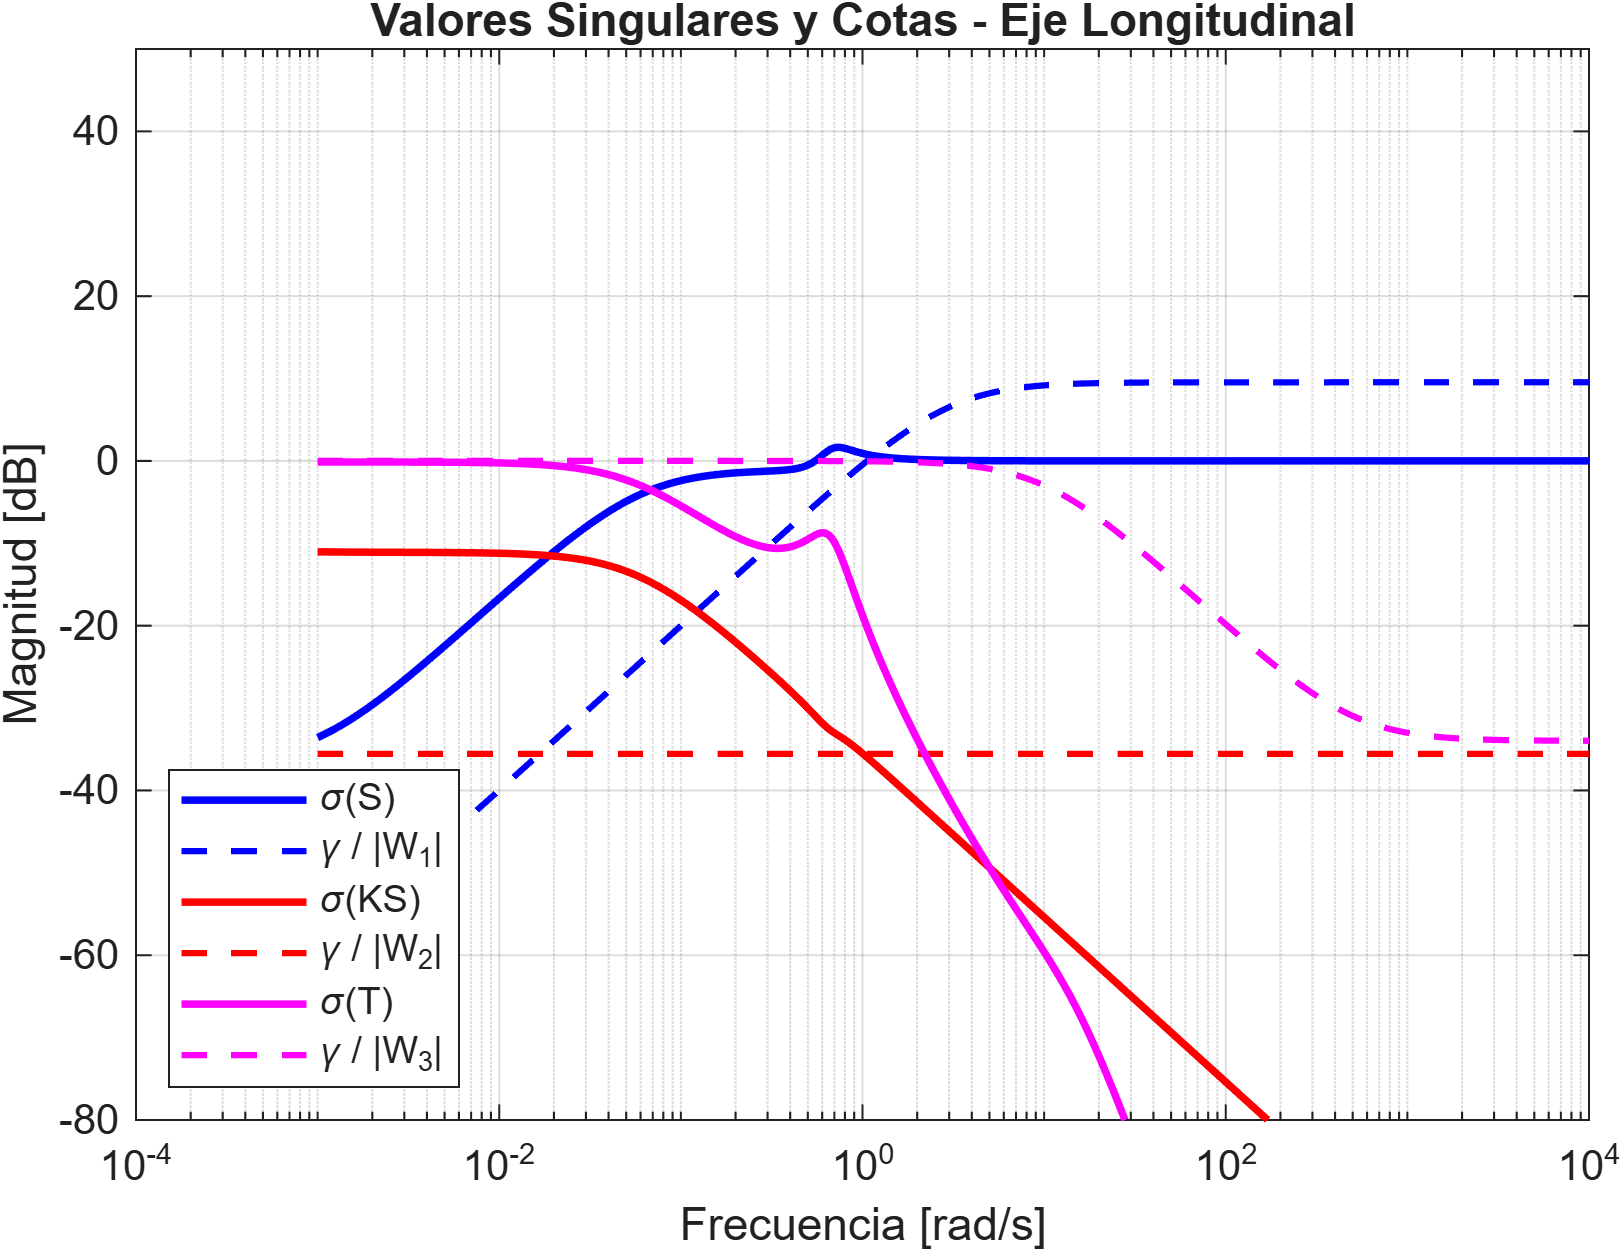
\includegraphics[height=3.35cm,width=\linewidth,keepaspectratio]{hinf_long_sigma.png}
    \caption{Valores singulares $\sigma$ y cotas inversas.}
    \label{fig:hinf_long_sigma}
  \end{subfigure}\hfill
  \begin{subfigure}[b]{0.48\linewidth}
    \centering
    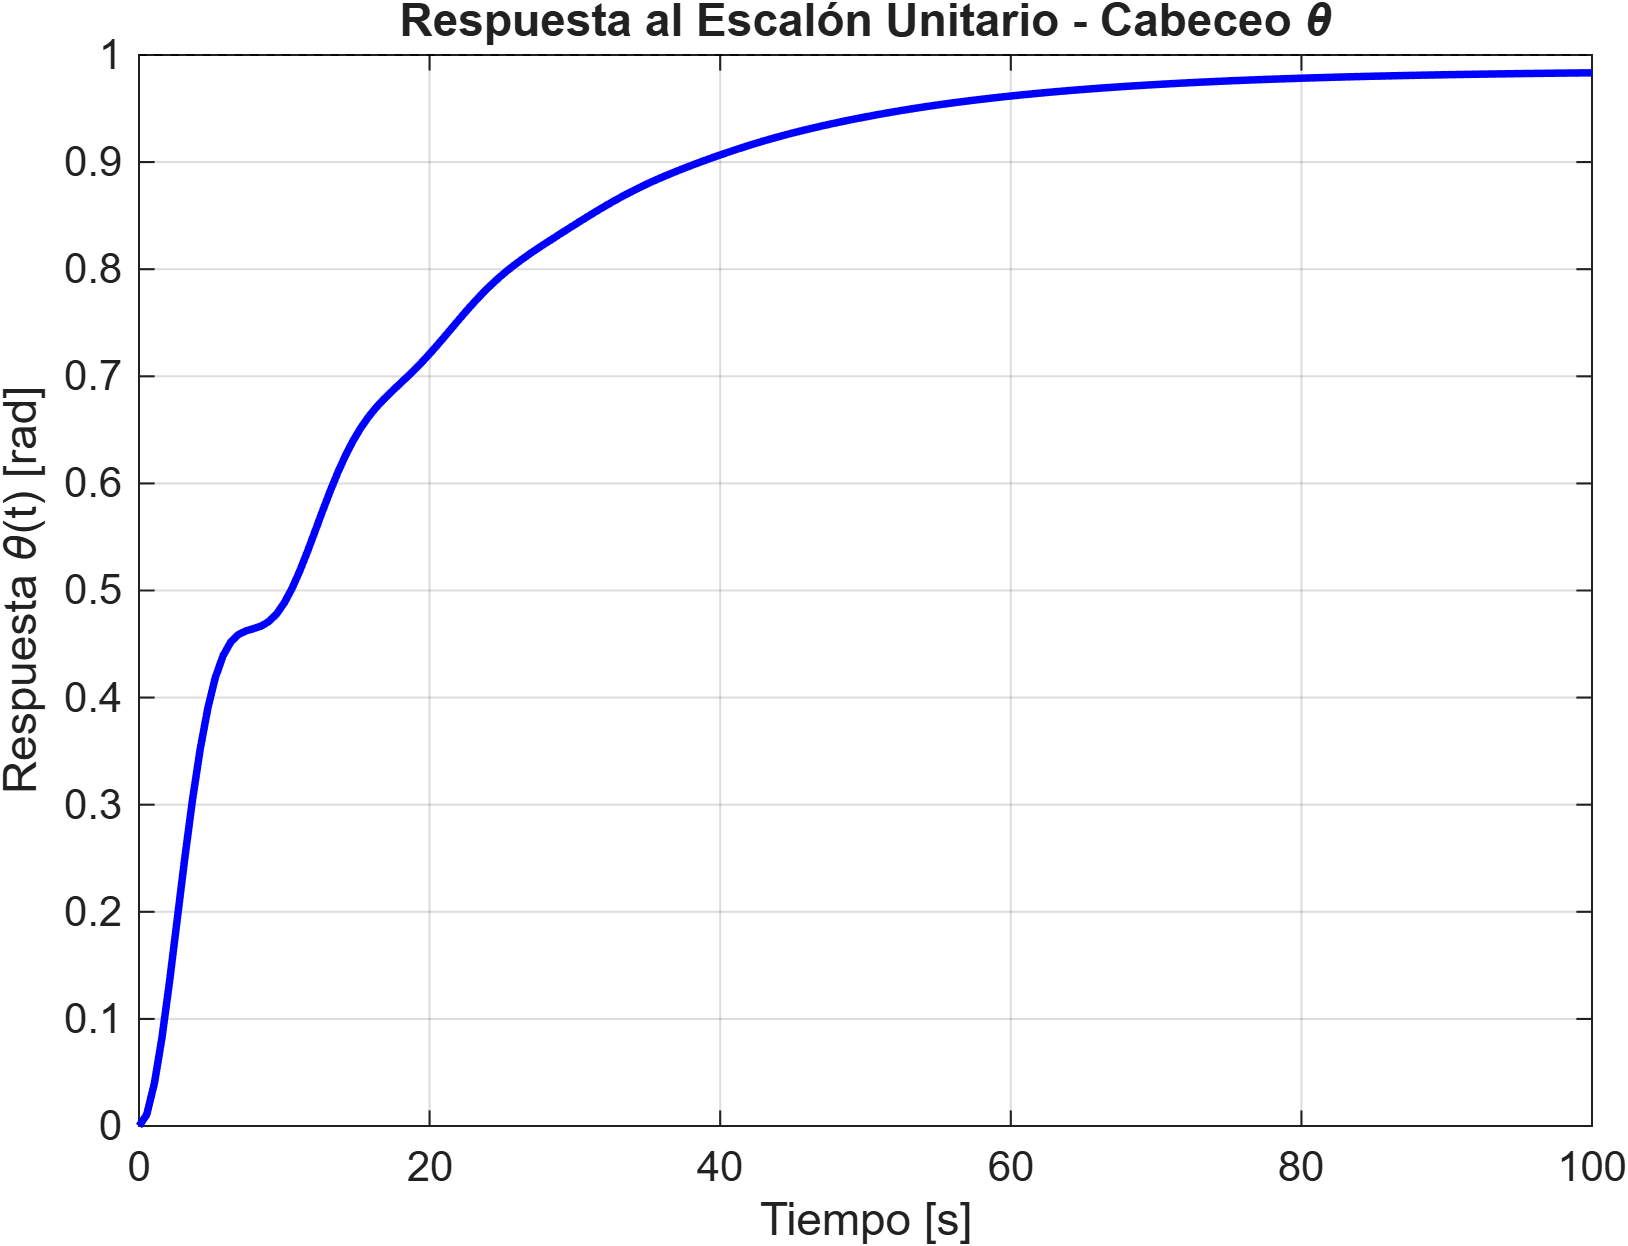
\includegraphics[height=3.35cm,width=\linewidth,keepaspectratio]{hinf_long_step.png}
    \caption{Respuesta temporal al escal\'on en $\theta$.}
    \label{fig:hinf_long_step}
  \end{subfigure}
  \vspace{-2mm}
  \caption{Desempe\~no $\mathcal{H}_\infty$ -- canal longitudinal ($\gamma = 58{,}12$, orden 8).}
  \label{fig:hinf_long}
\end{figure}

\analisis
El peso $W_2 = 60$ prioriza estrictamente evitar la saturaci\'on del elevador: con $\|KS\|_\infty = 0{,}9652$, ante una referencia de $40^\circ$ ($0{,}698\,\text{rad}$), el pico m\'aximo de control es $|\delta_e| \approx 38^\circ$. La respuesta es monot\'onica, libre de sobrepaso y cr\'iticamente amortiguada, intercambiando ancho de banda por preservaci\'on del actuador.

% -----------------------------------------------------------
\subsection{Dise\~no para eje direccional (Yaw)}
% -----------------------------------------------------------

\desarrollo
Para el canal direccional las salidas son la tasa de gui\~nada $r$ y el \'angulo de gui\~nada $\psi$ ($y = [r, \psi]^T$), actuados por el tim\'on $\delta_r$. Para garantizar la regularidad num\'erica se asigna una ponderaci\'on residual ($10^{-5}$) en la medida auxiliar $r$:
\begin{equation}
  W_1 = \operatorname{diag}(10^{-5},\, W_{1\psi}),\ W_{1\psi} = \frac{0{,}588\,s + 0{,}5}{s + 0{,}005}; \quad
  W_2 = 2; \quad
  W_3 = \operatorname{diag}(10^{-5},\, W_{3\psi}),\ W_{3\psi} = \frac{5\,s + 1885}{s + 2639}
\end{equation}
con $M_1 = 1{,}7$, $A_1 = 0{,}01$, $\omega_{b1} = 0{,}5\,\text{rad/s}$, $M_3 = 0{,}2$, $A_3 = 1{,}4$ y $\omega_{b3} = 2\pi(300)\,\text{rad/s}$.

\resultados
La s\'intesis alcanza un valor casi \'optimo $\gamma = 1{,}0531 \approx 1{,}0$ con un controlador de orden 11. La respuesta al escal\'on en $\psi$ no tiene sobrepaso ($M_p = 0{,}00\%$), con $t_r = 2{,}19\,\text{s}$ y $t_s = 4{,}34\,\text{s}$. El ancho de banda es $\omega_{BW} = 1{,}0212\,\text{rad/s}$ ($0{,}1625\,\text{Hz}$), con picos de norma $\|S_\psi\|_\infty = 1{,}3126$, $\|KS\|_\infty = 0{,}4362$ y $\|T_\psi\|_\infty = 1{,}0000$.

\begin{figure}[H]
  \centering
  \begin{subfigure}[b]{0.48\linewidth}
    \centering
    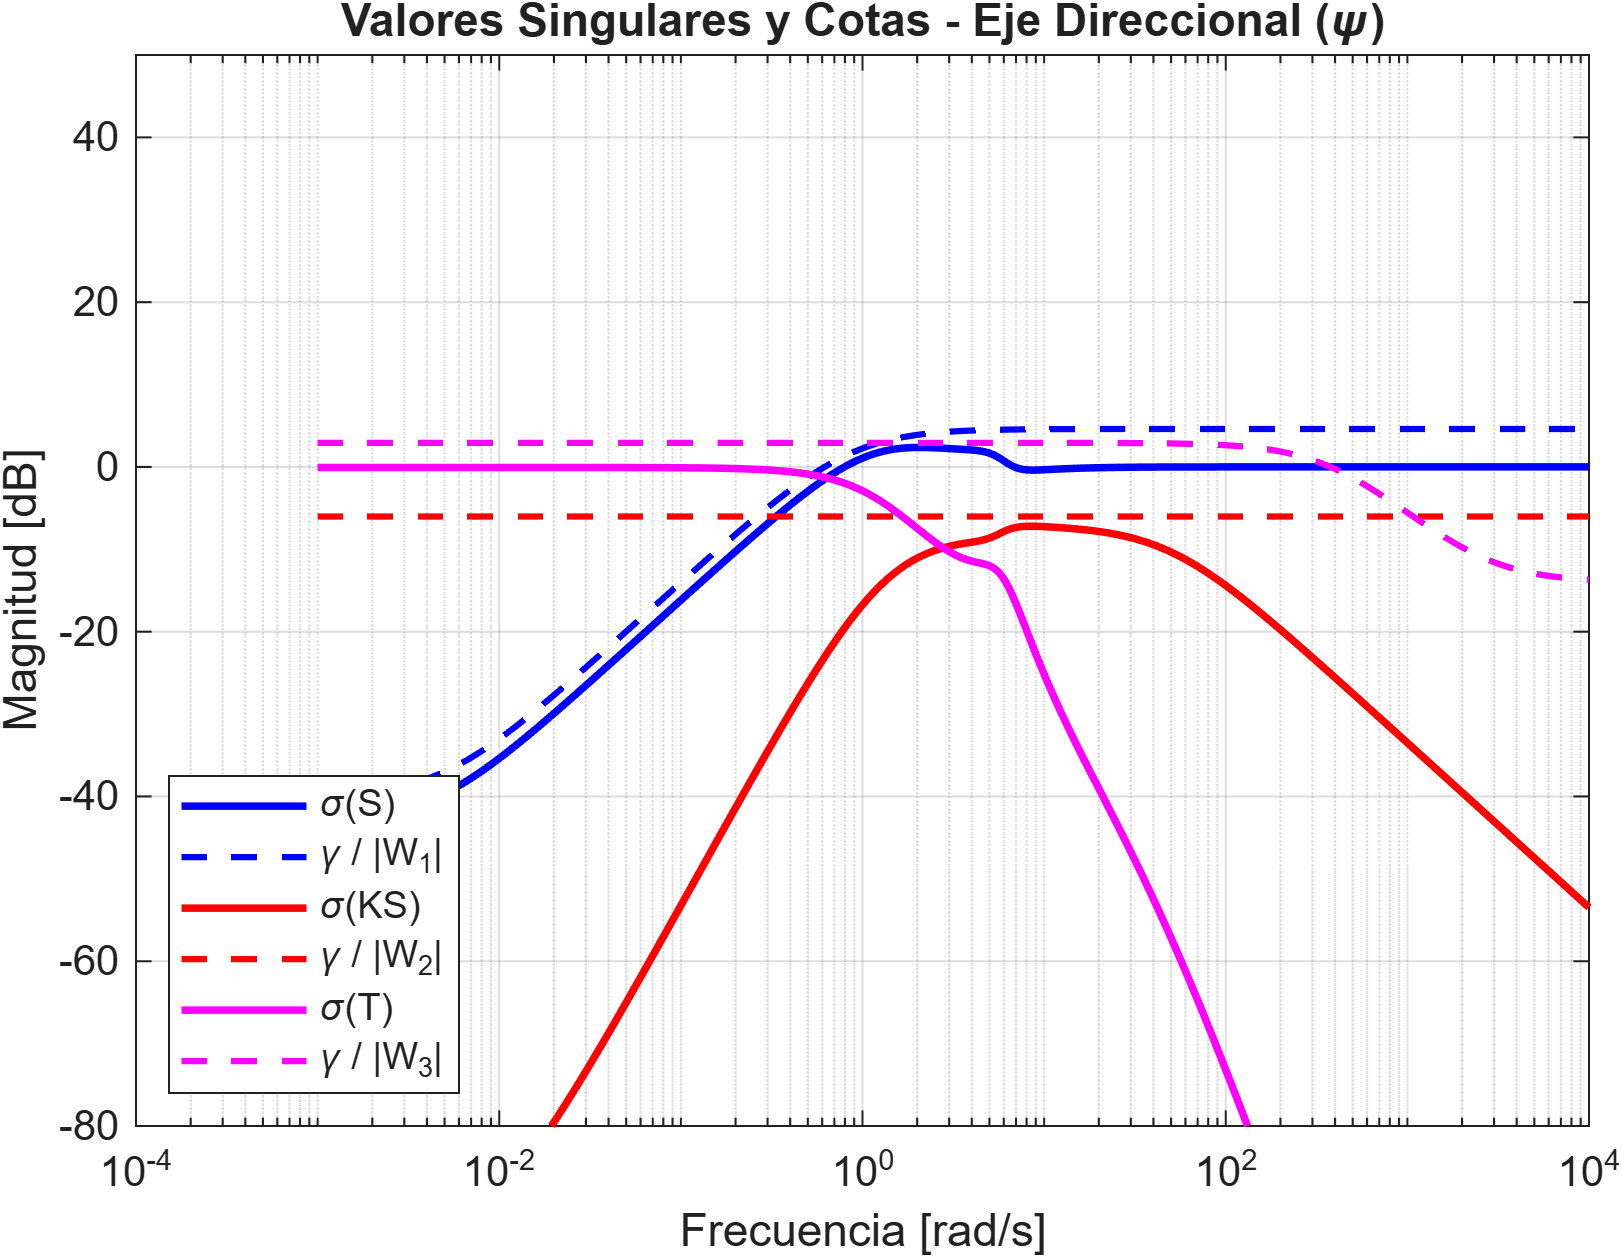
\includegraphics[height=3.35cm,width=\linewidth,keepaspectratio]{hinf_yaw_sigma.png}
    \caption{Valores singulares $\sigma$ y cotas inversas.}
    \label{fig:hinf_yaw_sigma}
  \end{subfigure}\hfill
  \begin{subfigure}[b]{0.48\linewidth}
    \centering
    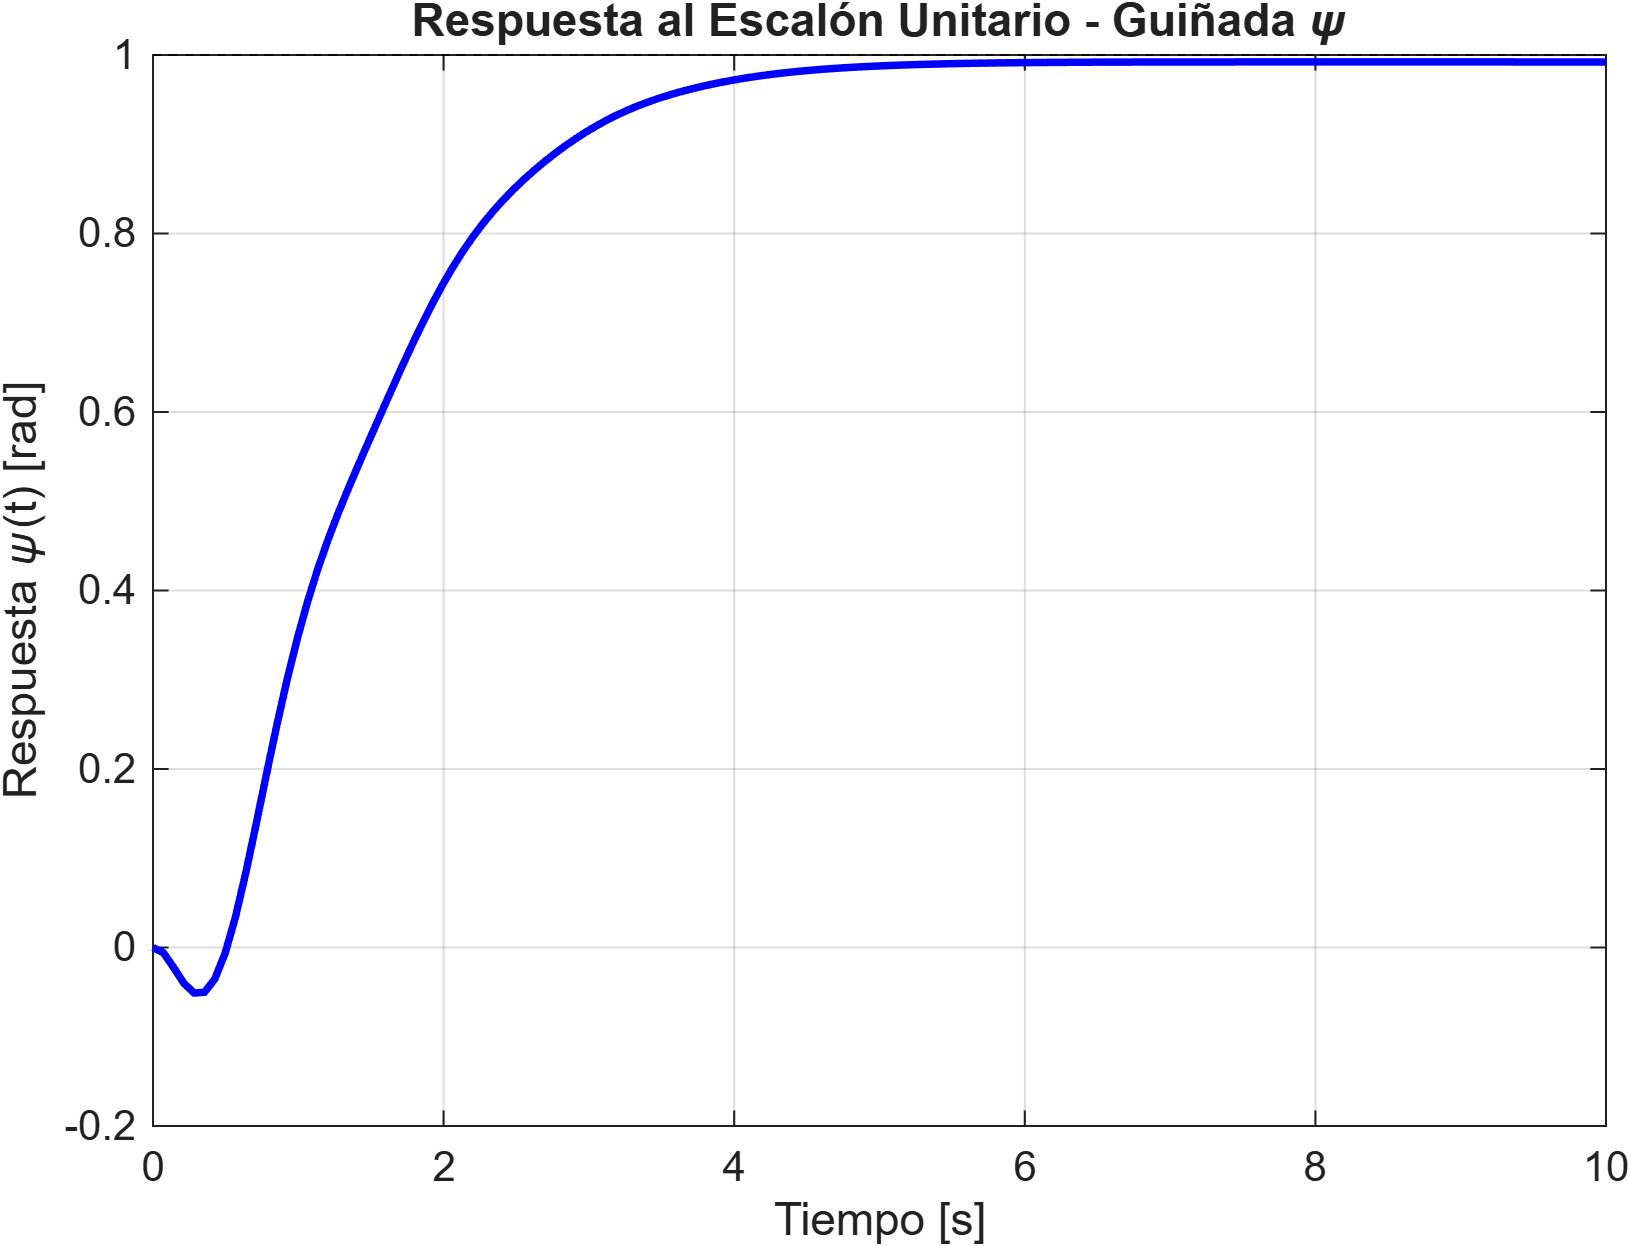
\includegraphics[height=3.35cm,width=\linewidth,keepaspectratio]{hinf_yaw_step.png}
    \caption{Respuesta temporal al escal\'on en $\psi$.}
    \label{fig:hinf_yaw_step}
  \end{subfigure}
  \vspace{-2mm}
  \caption{Desempe\~no $\mathcal{H}_\infty$ -- canal direccional ($\gamma = 1{,}0531$, orden 11).}
  \label{fig:hinf_yaw}
\end{figure}

\analisis
El controlador $\mathcal{H}_\infty$ supera categ\'oricamente al esquema $PI+D$: mientras este \'ultimo amplificaba la acci\'on de control hasta $\|KS\|_\infty = 301{,}17$ (inviable ante ruido), $\mathcal{H}_\infty$ reduce la norma a $0{,}4362$ (atenuaci\'on de casi 700 veces) y establece el sistema en $4{,}34\,\text{s}$ sin oscilaciones transitorias.

% -----------------------------------------------------------
\subsection{Dise\~no para eje lateral (Roll)}
% -----------------------------------------------------------

\desarrollo
El canal lateral desacoplado emplea las salidas de alabeo $p$ y $\phi$ ($y = [p, \phi]^T$) con entrada de aler\'on $\delta_a$. Los filtros sintonizados son:
\begin{equation}
  W_1 = \operatorname{diag}(0,\, W_{1\phi}),\ W_{1\phi} = \frac{0{,}667\,s + 15}{s + 0{,}015}; \quad
  W_2 = 5; \quad
  W_3 = \operatorname{diag}(0,\, W_{3\phi}),\ W_{3\phi} = \frac{50\,s + 628{,}3}{s + 628{,}3}
\end{equation}
con $M_1 = 1{,}5$, $A_1 = 10^{-3}$, $\omega_{b1} = 15\,\text{rad/s}$, $M_3 = 0{,}02$, $A_3 = 1$ y $\omega_{b3} = 2\pi(100)\,\text{rad/s}$.

\resultados
El \'indice obtenido es $\gamma = 3{,}4370$, resultando en un controlador de orden 6. La din\'amica es altamente reactiva y amortiguada: $M_p = 0{,}48\%$, $t_r = 0{,}3779\,\text{s}$ y $t_s = 0{,}8780\,\text{s}$. El ancho de banda resultante es $\omega_{BW} = 6{,}1983\,\text{rad/s}$ ($0{,}9865\,\text{Hz} \approx 1\,\text{Hz}$), con $\|S_\phi\|_\infty = 1{,}1395$, $\|KS\|_\infty = 0{,}6726$ y $\|T_\phi\|_\infty = 0{,}9966$.

\begin{figure}[H]
  \centering
  \begin{subfigure}[b]{0.48\linewidth}
    \centering
    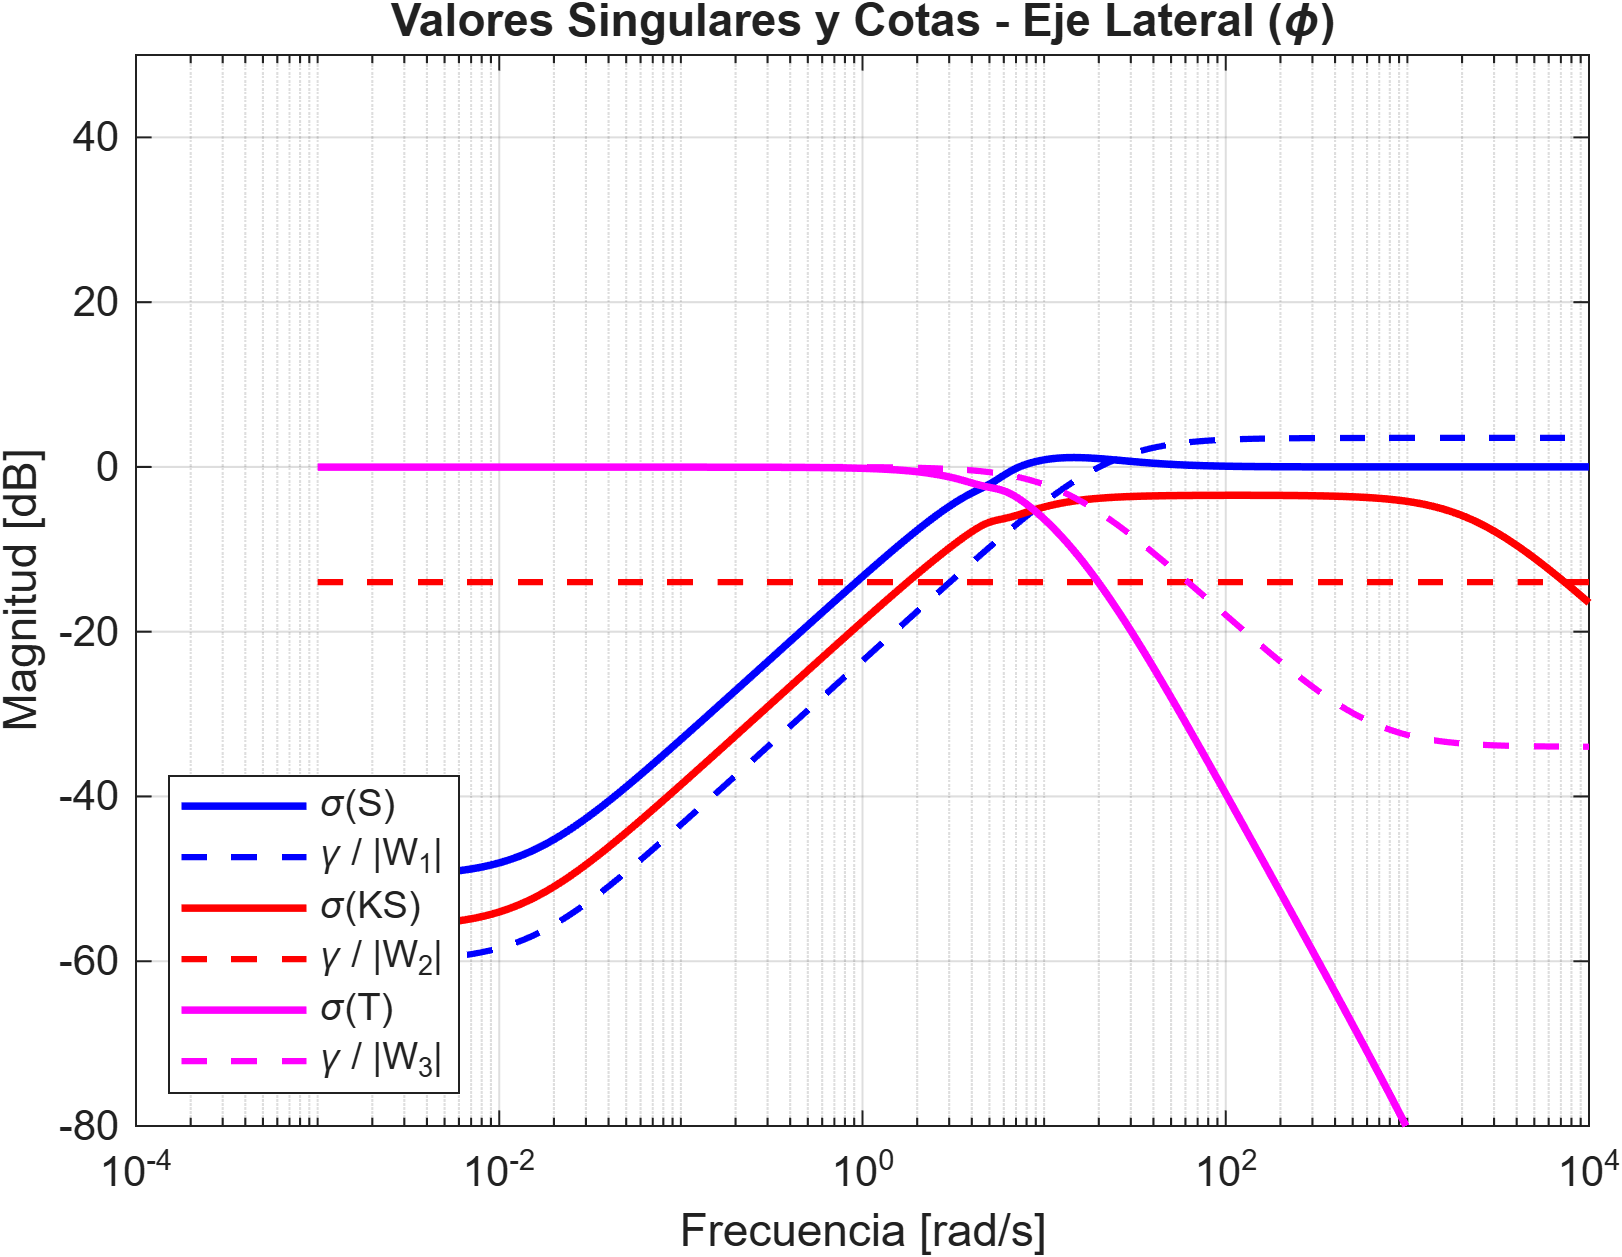
\includegraphics[height=3.35cm,width=\linewidth,keepaspectratio]{hinf_roll_sigma.png}
    \caption{Valores singulares $\sigma$ y cotas inversas.}
    \label{fig:hinf_roll_sigma}
  \end{subfigure}\hfill
  \begin{subfigure}[b]{0.48\linewidth}
    \centering
    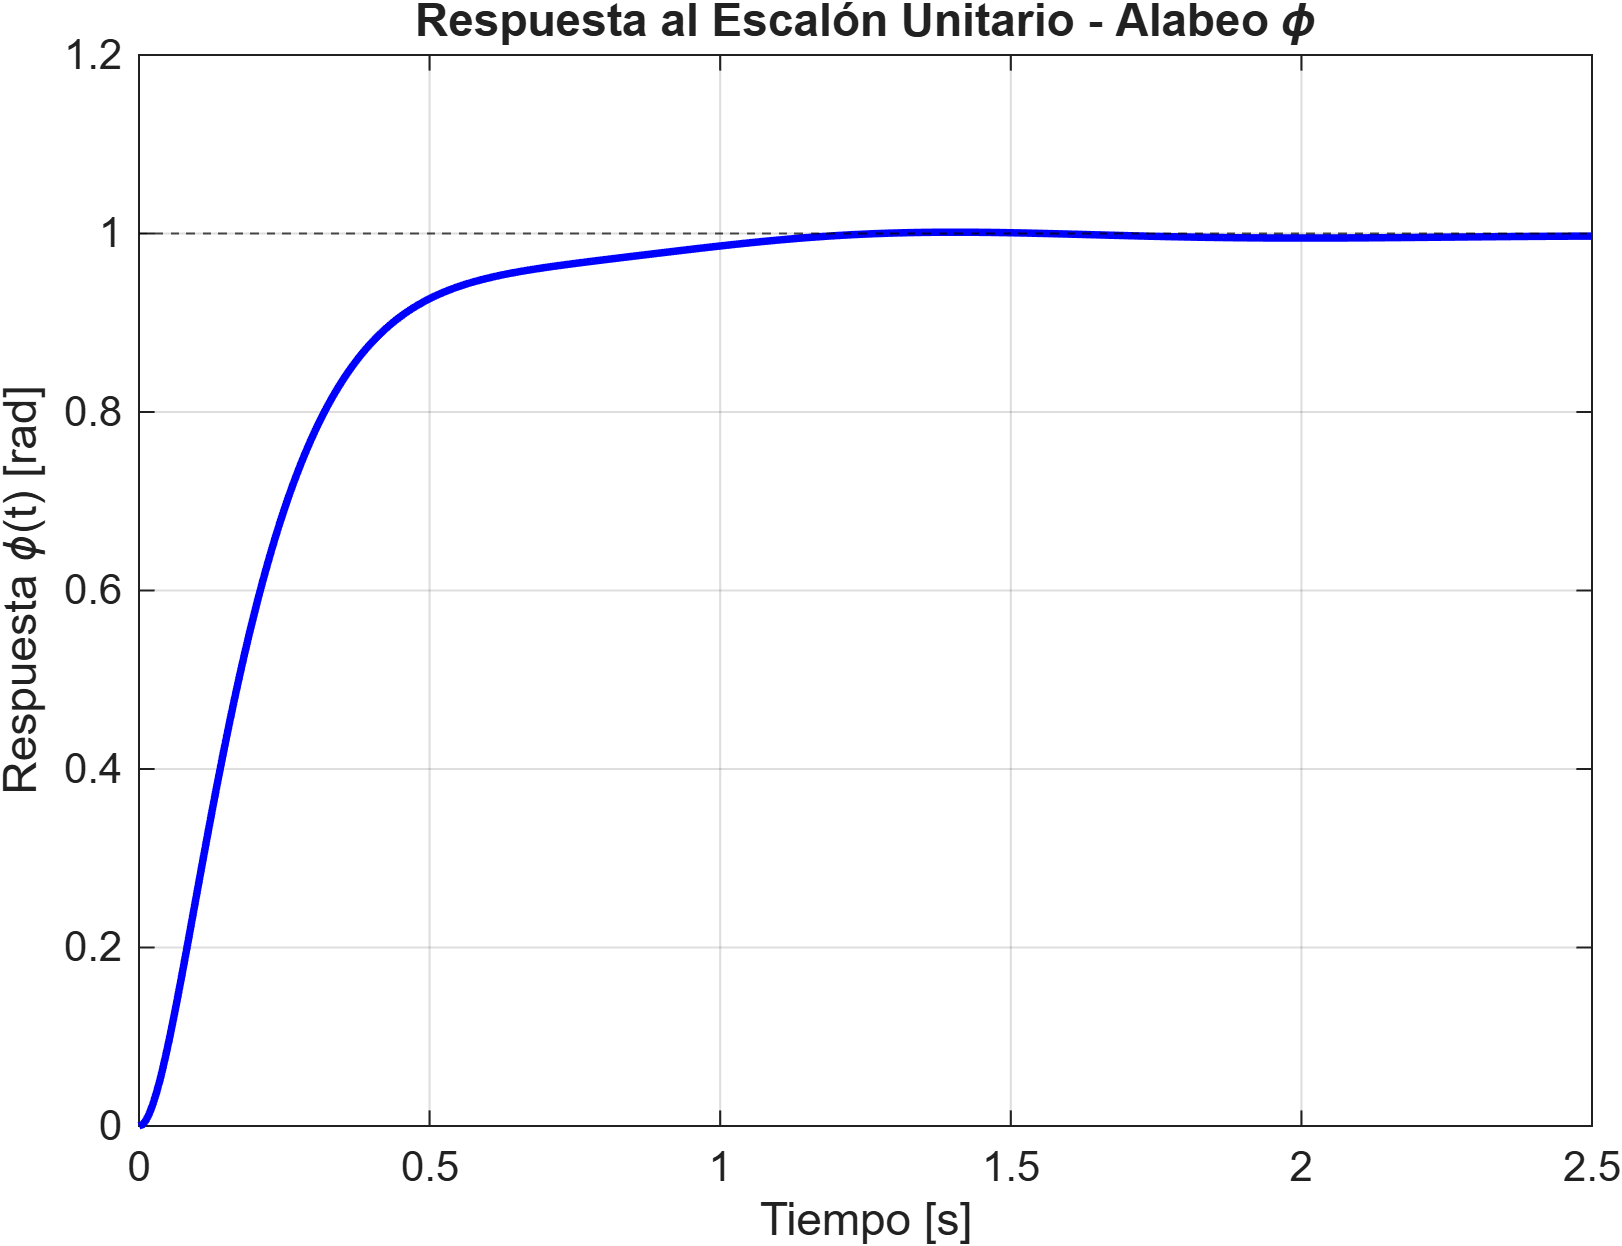
\includegraphics[height=3.35cm,width=\linewidth,keepaspectratio]{hinf_roll_step.png}
    \caption{Respuesta temporal al escal\'on en $\phi$.}
    \label{fig:hinf_roll_step}
  \end{subfigure}
  \vspace{-2mm}
  \caption{Desempe\~no $\mathcal{H}_\infty$ -- canal lateral ($\gamma = 3{,}4370$, orden 6).}
  \label{fig:hinf_roll}
\end{figure}

\analisis
El canal lateral evidencia la ventaja m\'as cr\'itica de $\mathcal{H}_\infty$: resuelve la incapacidad del $PI+D$ cl\'asico, el cual sufr\'ia un sobrepaso del $131{,}62\%$, tiempo de asentamiento de $662\,\text{s}$ y pico $\|S\|_\infty = 5{,}41$. $\mathcal{H}_\infty$ estabiliza los modos de balanceo en $0{,}88\,\text{s}$ con amortiguamiento cr\'itico ($M_p < 0{,}5\%$) y acci\'on moderada ($\|KS\|_\infty = 0{,}67$).

% -----------------------------------------------------------
\subsection{Comparaci\'on \texorpdfstring{$PI+D$ vs.\ $\mathcal{H}_\infty$}{PI+D vs. H-infinito}}
% -----------------------------------------------------------

La Tabla~\ref{tab:comparacion} recopila los indicadores comparativos de desempe\~no nominal y robustez para ambos esquemas.

\begin{table}[H]
  \centering
  \caption{Comparaci\'on cuantitativa de controladores por canal.}
  \label{tab:comparacion}
  \renewcommand{\arraystretch}{1.2}
  \small
  \begin{tabular}{llccccc}
    \toprule
    \textbf{Canal} & \textbf{Controlador}
      & $\omega_{BW}$ [Hz]
      & $M_p$ [\%]
      & $t_s$ [s]
      & $\|S\|_\infty$
      & $\|KS\|_\infty$ \\
    \midrule
    \multirow{2}{*}{Longitudinal}
      & $PI+D$              & $8{,}01$ & $7{,}40$  & $0{,}62$  & $1{,}21$ & $38{,}44$ \\
      & $\mathcal{H}_\infty$ & $0{,}01$ & $0{,}00$  & $74{,}09$ & $1{,}21$ & $0{,}97$ \\
    \midrule
    \multirow{2}{*}{Direccional}
      & $PI+D$              & $8{,}11$ & $7{,}13$  & $4{,}94$  & $1{,}09$ & $301{,}17$ \\
      & $\mathcal{H}_\infty$ & $0{,}16$ & $0{,}00$  & $4{,}34$  & $1{,}31$ & $0{,}44$ \\
    \midrule
    \multirow{2}{*}{Lateral}
      & $PI+D$              & $0{,}24$ & $131{,}62$ & $662{,}33$ & $5{,}41$ & $0{,}40$ \\
      & $\mathcal{H}_\infty$ & $0{,}99$ & $0{,}48$   & $0{,}88$   & $1{,}14$ & $0{,}67$ \\
    \bottomrule
  \end{tabular}
\end{table}

\begin{itemize}[leftmargin=*,noitemsep]
  \item \textbf{Esfuerzo de control y ruido:} El $PI+D$ exige ganancias excesivas ($\|KS\|_\infty$ hasta $301{,}2$), inviables ante ruido sensorial. $\mathcal{H}_\infty$ restringe $\|KS\|_\infty < 1$ en todos los canales.
  \item \textbf{Amortiguamiento cr\'itico:} $\mathcal{H}_\infty$ erradica sobrepasos transitorios ($M_p \leq 0{,}48\%$), cumpliendo la especificaci\'on de respuesta cr\'iticamente amortiguada.
  \item \textbf{Estabilidad lateral:} $\mathcal{H}_\infty$ reubica multivariablemente los polos donde el lazo cl\'asico diverge en oscilaciones prolongadas.
\end{itemize}

% ============================================================
\section*{Conclusiones}
% ============================================================

\begin{enumerate}[leftmargin=*,noitemsep]
  \item La s\'intesis $\mathcal{H}_\infty$ por sensibilidad mixta permiti\'o incorporar de forma expl\'icita el compromiso entre seguimiento, rechazo de perturbaciones y protecci\'on contra saturaci\'on ($|\delta| \leq 30^\circ$).
  \item El controlador robusto erradica la amplificaci\'on excesiva de ruido observada en el $PI+D$ ($\|KS\|_\infty$ reducido de $301{,}2$ a $0{,}44$ en gui\~nada) y resuelve la severa deficiencia lateral cl\'asica ($M_p$ reducido de $131{,}6\%$ a $0{,}48\%$).
  \item Aunque el esquema cl\'asico alcanza mayor ancho de banda longitudinal, la estrategia $\mathcal{H}_\infty$ garantiza amortiguamiento cr\'itico y operaci\'on acotada, imprescindible para la integridad f\'isica del UAV.
\end{enumerate}

\end{document}
